\chapter{Datenkompression}
\section{Huffman Codierung}
\subsubsection{Idee:}
Häufige Zeichen erhalten kurze Codewörter, seltene Zeichen längere Codewörter.
Gesucht ist ein Code, so dass die mittlere Codewortlänge minimal ist.
\subsubsection{Problem:}
Die Codierung muss eindeutig decodierbar sein.

\begin{shaded}
  \noindent
  \textbf{Def.:} Ein Präfixcode ist ein Code, bei dem kein Codewort Präfix eines anderen Codewortes ist.
\end{shaded}

\subsubsection{Beispiel}
\begin{center}
	\begin{tabular}{lcccccc}
		Zeichen & a & b & c & d & e & f\\
		Wahrscheinlichkeit & 0,45 & 0,13 & 0,12 & 0,16 & 0,09 & 0,05\\
		Code & 0 & 101 & 100 & 111 & 1101 & 1100
	\end{tabular}
\end{center}
Dieser Code ist optimal.
In Abbildung \ref{fig:HuffmanTree} ist der Code als Codewortbaum dargestellt.
\begin{figure}[htbp]
	\centering
	
\begin{tikzpicture}[sibling distance=5mm]
		\tikzstyle{end} = [circle, minimum width=4pt,fill, inner sep=0pt]
		\Tree
		[.\node {};
			\edge node[auto=right] {0};
			[.a ]
			\edge node[auto=left] {1};
			[.\node[end] {};
				\edge node[auto=right] {0};
				[.\node[end] {};
					\edge node[auto=right] {0};
					[.c ]
					\edge node[auto=left] {1};
					[.b ]
				]
				\edge node[auto=left] {1};
				[.\node[end] {};
					\edge node[auto=right] {0};
					[.\node[end] {};
						\edge node[auto=right] {0};
						[.f ]
						\edge node[auto=left] {1};
						[.e ]
					]
					\edge node[auto=left] {1};
					[.d ]
				]
			]
		]
	\end{tikzpicture}
	\caption{Die Folge 1001010 lässt sich eindeutig decodieren zu cba}
	\label{fig:HuffmanTree}
\end{figure}
Der Huffman-Algorithmus ist ein Greedy-Algorithmus (wählt den nächsten Schritt nach der besten Wahrscheinlichkeit) der einen optimalen Präfix-Code konstruiert.

\subsection{Implementierung}
\begin{lstlisting}[language=java]
Initialisierung: Jedes Zeichen ist ein Baum mit einem Knoten.

while (mehr als ein Baum vorhanden)
	Verbinde zwei Baeume mit den beiden niedrigsten
	Wahrscheinlichkeiten zu einem neuen Baum,
	die Wahrscheinlichkeiteb addieren sich.
\end{lstlisting}
Ein effizente Implentierung verwendet einen Min-Heap.
Die Laufzeit beträgt daher:
\begin{itemize}
	\item Heap initialisieren: \(\mathcal{O}(n)\)
	\item In jedem Schritt: Zwei Bäume entfernen und neuen Baum hinzufügen: \(\mathcal{O}(\log n)\)
	\item Nach \(\mathcal{O}(n) +1\) Schitten ist der Codebaum konstruiert
\end{itemize}
Die Laufzeit liegt daher in \(\mathcal{O}(n \log n)\)

\subsection{Optimalität des Huffman-Codes}
\begin{shaded}
  \noindent
  \textbf{Def.:} Für eine Wahrscheinlichkeitsverteilung mit den Massen \(p_1, \dots, p_n\) ist die Entropie wie folgt definiert:
	\[H(p_1, \dots, p_n) = -\sum_{k=1}^n p_k \log_2 p_k \]
	Sie gibt an wieviele Bits man benötigt um die Wörter zu codieren.
\end{shaded}
Für den Huffman-Code gilt:
\[H(p_1, \dots, p_n) \leq \text{mittlere Codewortlänge} \leq H(p_1, \dots, p_n)+1\]

\subsection{Beispiel}
\begin{figure}[htbp]
	\centering
	\begin{tikzpicture}[sibling distance=5mm]
		\node[state] 				(1)		{f};
		\node[above of=1] 			(11)	{0,05};
		\node[state, right of=1]	(2)		{e};
		\node[above of=2] 			(21)	{0,09};
		\node[state, right of=2]	(3)		{c};
		\node[above of=3] 			(31)	{0,12};
		\node[state, right of=3]	(4)		{b};
		\node[above of=4] 			(41)	{0,13};
		\node[state, right of=4]	(5)		{d};
		\node[above of=5] 			(51)	{0,16};
		\node[state, right of=5]	(6)		{a};
		\node[above of=6] 			(61)	{0,45};
	\end{tikzpicture}
\end{figure}

\begin{center}
	\begin{tabular}{llll}
		% 1. Zeile
		\begin{tikzpicture}[sibling distance=5mm]
			\node[state]				(3)		{c};
			\node[above of=3] 			(11)	{0,12};
			\node[state, right of=3]	(4)		{b};
			\node[above of=4] 			(11)	{0,13};
		\end{tikzpicture}
		&
		\multicolumn{2}{c}{
			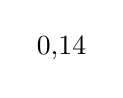
\begin{tikzpicture}[sibling distance=10mm]
				\tikzstyle{end} = [circle, minimum width=4pt,fill, inner sep=0pt]
				\Tree
				[.\node {0,14};
					\edge node[auto=right] {0};
					[.f ]
					\edge node[auto=left] {1};
					[.e ]
				]
			\end{tikzpicture}
		}
		&
		\begin{tikzpicture}[sibling distance=5mm]
			\node[state]	(5)		{d};
			\node[above of=5] 			(11)	{0,16};
			\node[state, right of=5]	(6)		{a};
			\node[above of=6] 			(11)	{0,45};
		\end{tikzpicture}
		\vspace{1cm}
		\\ 
		% 2. Zeile
		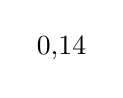
\begin{tikzpicture}[sibling distance=10mm]
			\tikzstyle{end} = [circle, minimum width=4pt,fill, inner sep=0pt]
			\Tree
			[.\node {0,14};
				\edge node[auto=right] {0};
				[.f ]
				\edge node[auto=left] {1};
				[.e ]
			]
		\end{tikzpicture}
		& 
		\begin{tikzpicture}[sibling distance=5mm]
			\node[state]				(3)		{d};
			\node[above of=3] 			(31)	{0,16};
		\end{tikzpicture}
		& 
		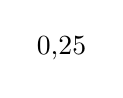
\begin{tikzpicture}[sibling distance=10mm]
			\tikzstyle{end} = [circle, minimum width=4pt,fill, inner sep=0pt]
			\Tree
			[.\node {0,25};
				\edge node[auto=right] {0};
				[.c ]
				\edge node[auto=left] {1};
				[.b ]
			]
		\end{tikzpicture}
		&
		\begin{tikzpicture}[sibling distance=5mm]
			\node[state]				(3)		{a};
			\node[above of=3] 			(31)	{0,45};
		\end{tikzpicture}
		\vspace{1cm}
		\\
		% 3. Zeile
		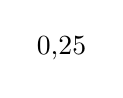
\begin{tikzpicture}[sibling distance=10mm]
			\tikzstyle{end} = [circle, minimum width=4pt,fill, inner sep=0pt]
			\Tree
			[.\node {0,25};
				\edge node[auto=right] {0};
				[.c ]
				\edge node[auto=left] {1};
				[.b ]
			]
		\end{tikzpicture}
		&
		\multicolumn{2}{c}{
			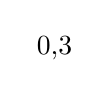
\begin{tikzpicture}[sibling distance=5mm]
				\tikzstyle{end} = [circle, minimum width=4pt,fill, inner sep=0pt]
				\Tree
				[.\node {0,3};
					\edge node[auto=right] {0};
					[ \edge node[auto=right] {0};
						[.f ]
						\edge node[auto=left] {1};
						[.e ]
					]
					\edge node[auto=left] {1};
					[.d ]
				]
			\end{tikzpicture}
		}
		&
		\begin{tikzpicture}[sibling distance=5mm]
			\node[state]				(3)		{a};
			\node[above of=3] 			(31)	{0,45};
		\end{tikzpicture}
	\end{tabular}
\end{center}

\begin{center}
	\begin{tabular}{llll}
		% 4. Zeile
		\begin{tikzpicture}[sibling distance=5mm]
			\node[state]				(3)		{a};
			\node[above of=3] 			(31)	{0,45};
		\end{tikzpicture}
		&
		\multicolumn{3}{c}{
			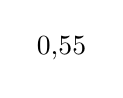
\begin{tikzpicture}[sibling distance=5mm]
				\tikzstyle{end} = [circle, minimum width=4pt,fill, inner sep=0pt]
				\Tree
				[.\node {0,55};
					\edge node[auto=right] {0};
					[
						\edge node[auto=right] {0};
						[.c ]
						\edge node[auto=left] {1};
						[.b ]
					]
					\edge node[auto=left] {1};
					[
						\edge node[auto=right] {0};
						[
							\edge node[auto=right] {0};
							[.f ]
							\edge node[auto=left] {1};
							[.e ]
						]
						\edge node[auto=left] {1};
						[.d ] ]
				]
			\end{tikzpicture}
		}
	\end{tabular}
\end{center}
Das Ergbiss ist:
\begin{center}
	\begin{tikzpicture}[sibling distance=5mm]
		\tikzstyle{end} = [circle, minimum width=4pt,fill, inner sep=0pt]
		\Tree
		[.\node {};
			\edge node[auto=right] {0};
			[.a ]
			\edge node[auto=left] {1};
			[
				\edge node[auto=right] {0};
				[
					\edge node[auto=right] {0};
					[.c ]
					\edge node[auto=left] {1};
					[.b ]
				]
				\edge node[auto=left] {1};
				[
					\edge node[auto=right] {0};
					[
						\edge node[auto=right] {0};
						[.f ]
						\edge node[auto=left] {1};
						[.e ]
					]
					\edge node[auto=left] {1};
					[.d ] ]
			]
		]
	\end{tikzpicture}
\end{center}
